\documentclass[main]{subfiles}
\begin{document}

%@@@@@@@@@@@@@@@@@@@@@@@@@@@@@@
\noindent
\textbf{Topics: Feed-Forward Networks and Backpropagation - 05.12.2019} \\
Lecturer: Dr. Matthew Cook \\
Author: Vanessa Leite \{vanessa at ini.uzh.ch\}

\section{Feed-Forward Networks}
\begin{itemize}[noitemsep,nolistsep]
	\item Multiple layers of neurons with a certain number of inputs and outputs.
	\item Every laxer of nodes feeds the next layer with inputs.
	\item There is an input and an output layer with hidden layers in between.
\end{itemize}

\begin{figure}[H]
	\centering
	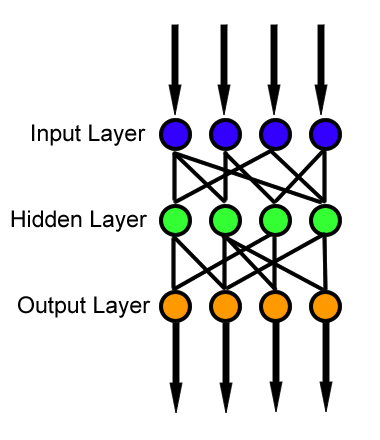
\includegraphics[width=0.25\textwidth]{Feed_forward_neural_net.png}
\end{figure}

\subsection{Boltzmann Machines}

\subsection{Backpropagation and Error function}
\begin{itemize}[noitemsep,nolistsep]
	\item The inputs and desired outputs are given as $S=\{(x,d)^1,\ldots,(x,d)^l\}$.
	\item The error function is given as $E(S) = \sum_i\frac{1}{2}||y(x^i)-d^i||^2$.
	\item The output is a non-linear transformation $y=f(a)$.
	\item $f(a)$ is the activation function, which is usually a sigmoid function.
	\item The error function for a single training sample is $E(S)=\frac{1}{2}(f(x_1w_1+x_2w_2+w_0)-d)^2$.
	\item The output of a simple network is for example $y(x_1,x_2,x_3)=f(x_1w_{21}+f(x_2w_{11}+x_3w_{12}+w_{10})w_{22}+w_{20})$.
	\item $\frac{\partial E(w_1,w_2,w_0)}{\partial w_1}=(f(x_1w_1+x_2w_2+w_0)-d)\cdot f'(x_1w_1+x_2w_2+w_0)\cdot x_1$.
	\item $\frac{\partial E(w_1,w_2,w_0)}{\partial w_2}=(f(x_1w_1+x_2w_2+w_0)-d)\cdot f'(x_1w_1+x_2w_2+w_0)\cdot x_2$.
	\item $\frac{\partial E(w_1,w_2,w_0)}{\partial w_0}=(f(x_1w_1+x_2w_2+w_0)-d)\cdot f'(x_1w_1+x_2w_2+w_0)$.
	\item The error terms travel backwards through the network and get multiplied with the derivative of the activation function of that input. Multiple error terms can just be added up.
	\item The partial derivative of the error $E$ term in relation to the weight $w$ to be adjusted can be added to the weight in order to learn. An additional weighting factor can be added.
\end{itemize}

\section{Signal Propagation in a Network}
\subsection{Avalanche Model}
\begin{itemize}[noitemsep,nolistsep]
	\item For example needed with sensory neurons, as smalls ignals have to be amplified in order to be detectable by the superior areas.
	\item No recurrent connections or risk of positive feedback with risk of explosion.
	\item $(pn)^2$ active neurons per layer. $p$ is a probability and $n$ is the number of neurons that every next layer has more than the previous ones. One neuron from the last layer is connected with $n$ from the next one.
\end{itemize}

\subsection{Synfire Chain}
\begin{itemize}[noitemsep,nolistsep]
	\item The synfire chain is a feedforward structure.
	\item Synchrony is the most important factor for the transmission of the signal.
	\item Noise is important: The chain is usually embedded in a larger network to transmit information. Introducing noise avoids that large-scale synchronization of neuronal firing contaminates the whole network.
\end{itemize}


\end{document}
